Another important aspect of the system is the way files are identified. 
Identification simply by file name is out of the picture. We can take as 
example two installers of the same applications, but each for a different 
version. This would cause a lot of collision possibilities, which is not 
desirable the file to identifier mapping has to be "as injective as possible." 
Another possibility would be to use a hashing function on the file contents. 
This is a good approach but, in theory, specials files can be crafted in such a 
way as its hash to match the hash of another file. To greatly increase the 
difficulty of such an endeavor, a combination of the file content hash and file 
size can be used. To further reduce the probability of eventual accidental 
collisions, the file name can be used as well. The combinations of these three 
values is called the \textit{augmented hash} of the file (or \textit{AHash} for 
short).

\begin{figure}
    \centering
    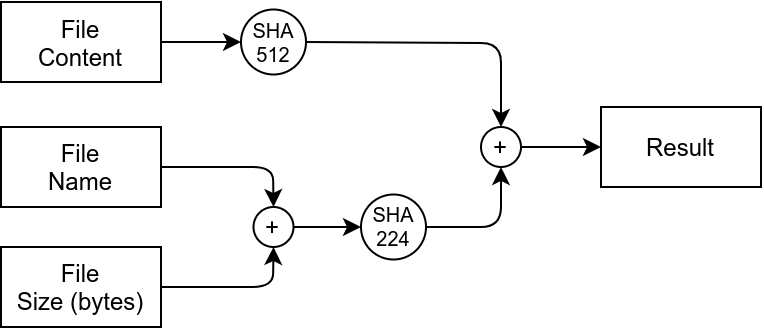
\includegraphics[width=0.7\textwidth]{figures/fig3}
    \caption{Obtaining the augmented hash (AHash)}
    \label{fig:fig3}
\end{figure}

Figure \ref{fig:fig3} illustrates the process of obtaining the AHash of a file. 
SHA-3-512 is used for hashing the file content. Because files have virtually no 
limit in size, the algorithm which reduces collisions the most is needed. File 
names and the string representation of the size are relatively short and thus 
SHA-3-224 is enough. The "+" sign means string concatenation. The final string 
will be 184 characters long.

The resulted AHash can be distributed on the internet, and other people may 
utilize it to search through the network for the distributed file.
